\documentclass[tikz,border=10pt]{standalone}
\usepackage{amsmath,amssymb}
\usepackage{tikz}
\usetikzlibrary{arrows,automata,backgrounds,calendar,chains,decorations,decorations.pathreplacing,decorations.text,fit,matrix,mindmap,patterns,petri,plotmarks,positioning,shadows,shapes,shapes.callouts,shapes.geometric,shapes.misc,spy,trees,calc,intersections,tikzmark,arrows.meta}
\usepackage{xcolor}
\usepackage{pgfplots}
\pgfplotsset{compat=1.16}

% Common math macros from the book
\def\x{\mathbf{x}}
\def\y{\mathbf{y}}
\def\z{\mathbf{z}}
\def\A{\mathbf{A}}
\def\b{\mathbf{b}}
\def\c{\mathbf{c}}
\def\w{\mathbf{w}}
\def\v{\mathbf{v}}
\def\u{\mathbf{u}}
\def\e{\mathbf{e}}
\def\zero{\mathbf{0}}
\def\R{\mathbb{R}}
\def\N{\mathbb{N}}
\def\Z{\mathbb{Z}}
\def\Q{\mathbb{Q}}
\def\st{\text{s.t.}}
\def\vect#1{\mathbf{#1}}
\def\xLP{x^{\mathrm{LP}}}
\def\zLP{z^{\mathrm{LP}}}
\def\xIP{x^{\mathrm{IP}}}

% Common node styles from the book
\tikzset{
    main/.style={circle, draw, fill=gray!20, minimum size=1cm, font=\normalsize},
    dot/.style={circle,fill=blue,minimum size=3pt,inner sep=0pt, outer sep=-1pt},
    vertex/.style={circle,fill=black!25,minimum size=20pt,inner sep=0pt},
    edge/.style={draw,-,thick},
    directed edge/.style={draw,->,>=latex,thick},
}

% Additional macros for 3D/coordinate systems
\newcommand{\xhat}{\hat{\x}}
\newcommand{\yhat}{\hat{\y}}
\newcommand{\zhat}{\hat{\z}}
\newcommand{\ihat}{\hat{\imath}}
\newcommand{\jhat}{\hat{\jmath}}
\newcommand{\khat}{\hat{k}}

\begin{document}
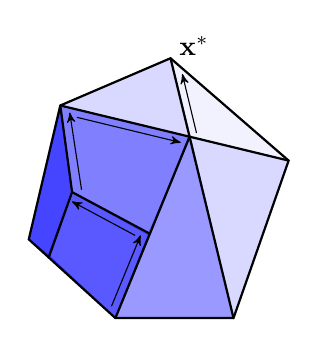
\begin{tikzpicture}[dot/.style={circle,fill=blue,minimum size=3pt,inner sep=0pt, outer sep=-1pt}, >=stealth']

    \draw[blue!10!, fill=blue!5!](3,1)--(1.5,2.3)--(1.75,1.3)--cycle;
    \draw[blue!25!, fill = blue!15!](3,1)--(1.75,1.3)--(2.3,-1)--cycle;
    \draw[blue!55!, fill = blue!40!](1.75,1.3)--(2.3,-1)--(.8,-1)--cycle;
    \draw[blue!80!, fill = blue!65!](.8,-1)--(-.05,-.2)--(.25,.6)--(1.22,.06)--cycle;
    \draw[blue!85!, fill = blue!73!](-.05, -.2)--(-.3,0)--(.1, 1.65)--(.25, .6)--cycle;
    \draw[blue!65!, fill = blue!50!](.1,1.7)--(.25,.6)--(1.22,.07)--(1.75,1.3)--cycle;
    \draw[blue!40!, fill = blue!15!](.1,1.7)--(1.75,1.3)--(1.5,2.3)--cycle;

    \draw[-,thick](-.3,0)--(.1,1.7)--(1.5, 2.3)--(3, 1)--(2.3,-1)--(.8,-1)--cycle;

    \draw[-,thick](.1,1.7)--(3,1);
    \draw[-,thick](1.5, 2.3)--(2.3,-1);
    \draw[-,thick](.8,-1)--(1.74,1.3);
    \draw[-,thick](.1,1.7)--(.25,.6);
    \draw[-,thick](1.24,.07)--(.25,.6);
    \draw[-,thick](-.05,-.24)--(.25,.6);

    \draw[->](.37,.63)--(.22,1.61);
    \draw[->](.31,1.55)--(1.63,1.23);
    \draw[->](.75,-.85)--(1.12,.05);
    \draw[->](1.05,.05)--(.25,.48);
    \draw[->](1.83,1.35)--(1.65,2.1);

    \node[draw=none](x*)at(1.8,2.45){$\x^*$};

    \end{tikzpicture}
\end{document}
